\chapter{Programación lineal}

\section{Objetivo de la programación lineal e interpretación en $\IR^3$}
El objetivo de la programación lineal es resolver el problema de
minimizar o maximizar una función $f:\IR^n\longrightarrow\IR$
restringida a un dominio $D\subset\IR^n$ de manera que tanto $f$ como
$D$ cumplan ciertas condiciones.

\begin{figure}[h]
  \caption{La función lineal $f(x,y)=2.5 - 0.5 x - 0.3 y$ restringida al plano $(x, y)$}
  \centering
  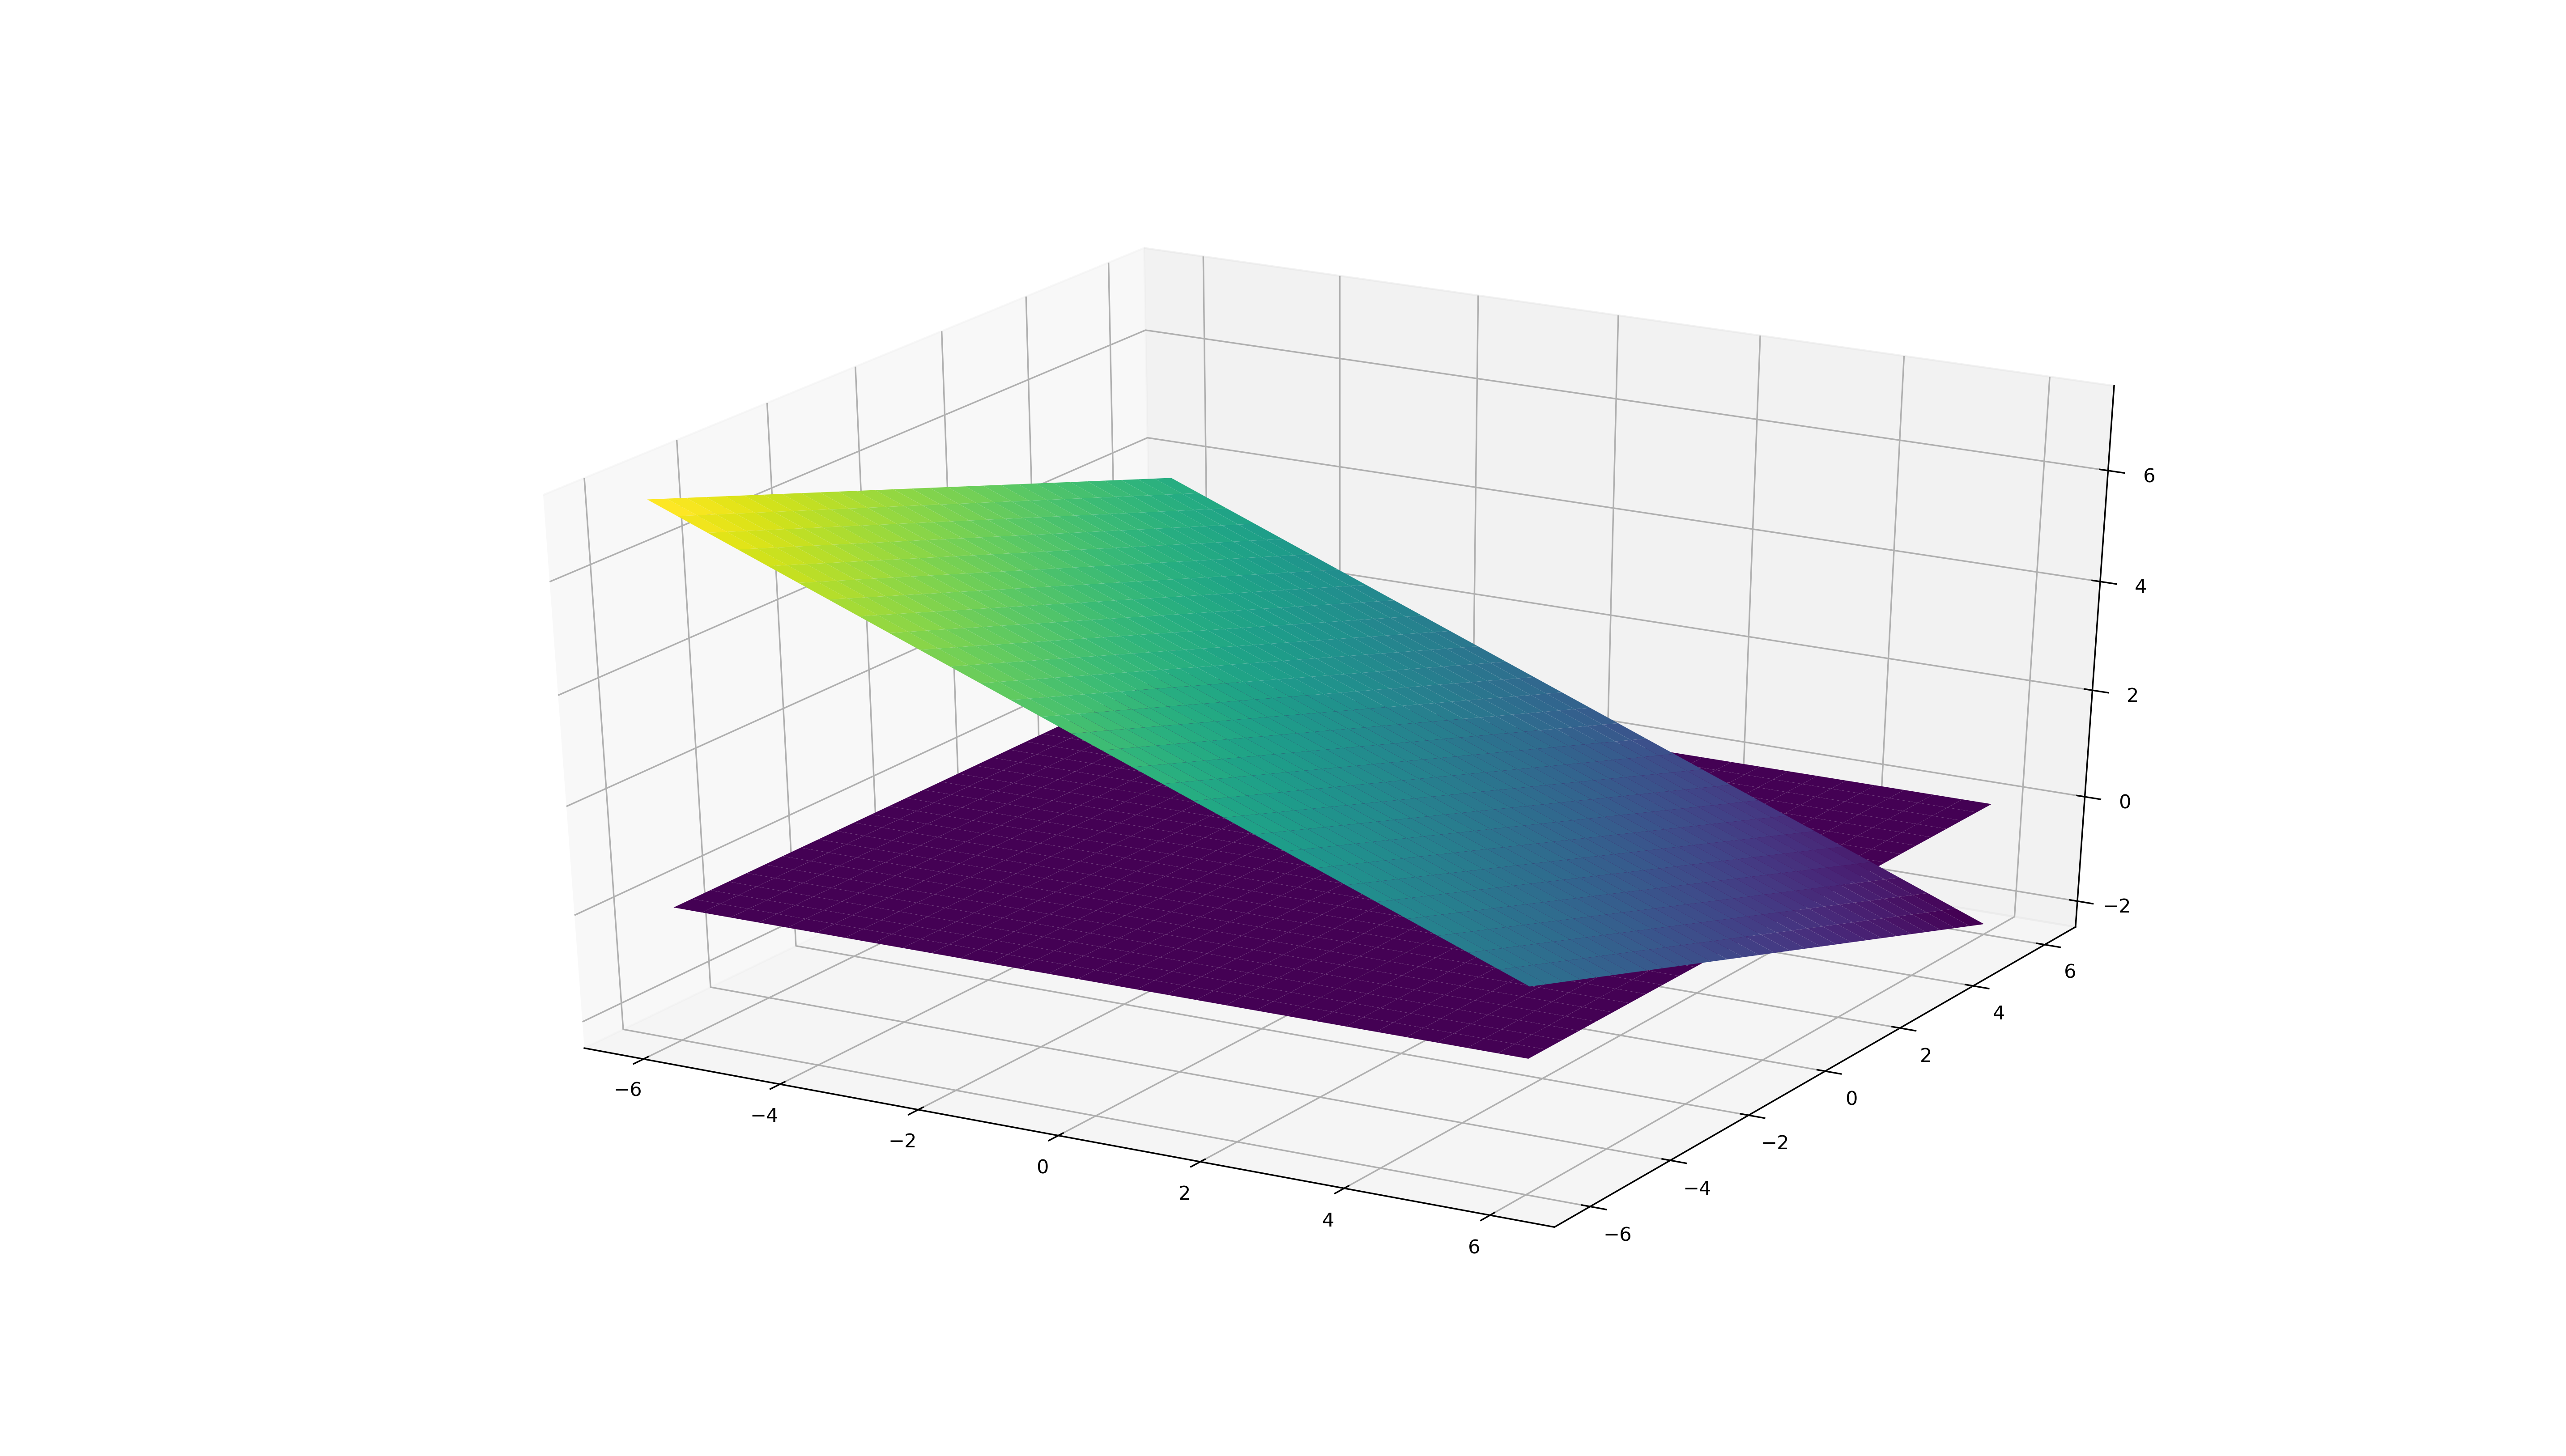
\includegraphics[width=\textwidth]{2_1_1.png}
\end{figure}

A la función $f:\IR^n\longrightarrow\IR$ se le pide que sea lineal y a $D$ que sea un conjunto definido por desigualdades lineales.
